\section{Opis implementacji}

\begin{figure}[!h]
	\center
	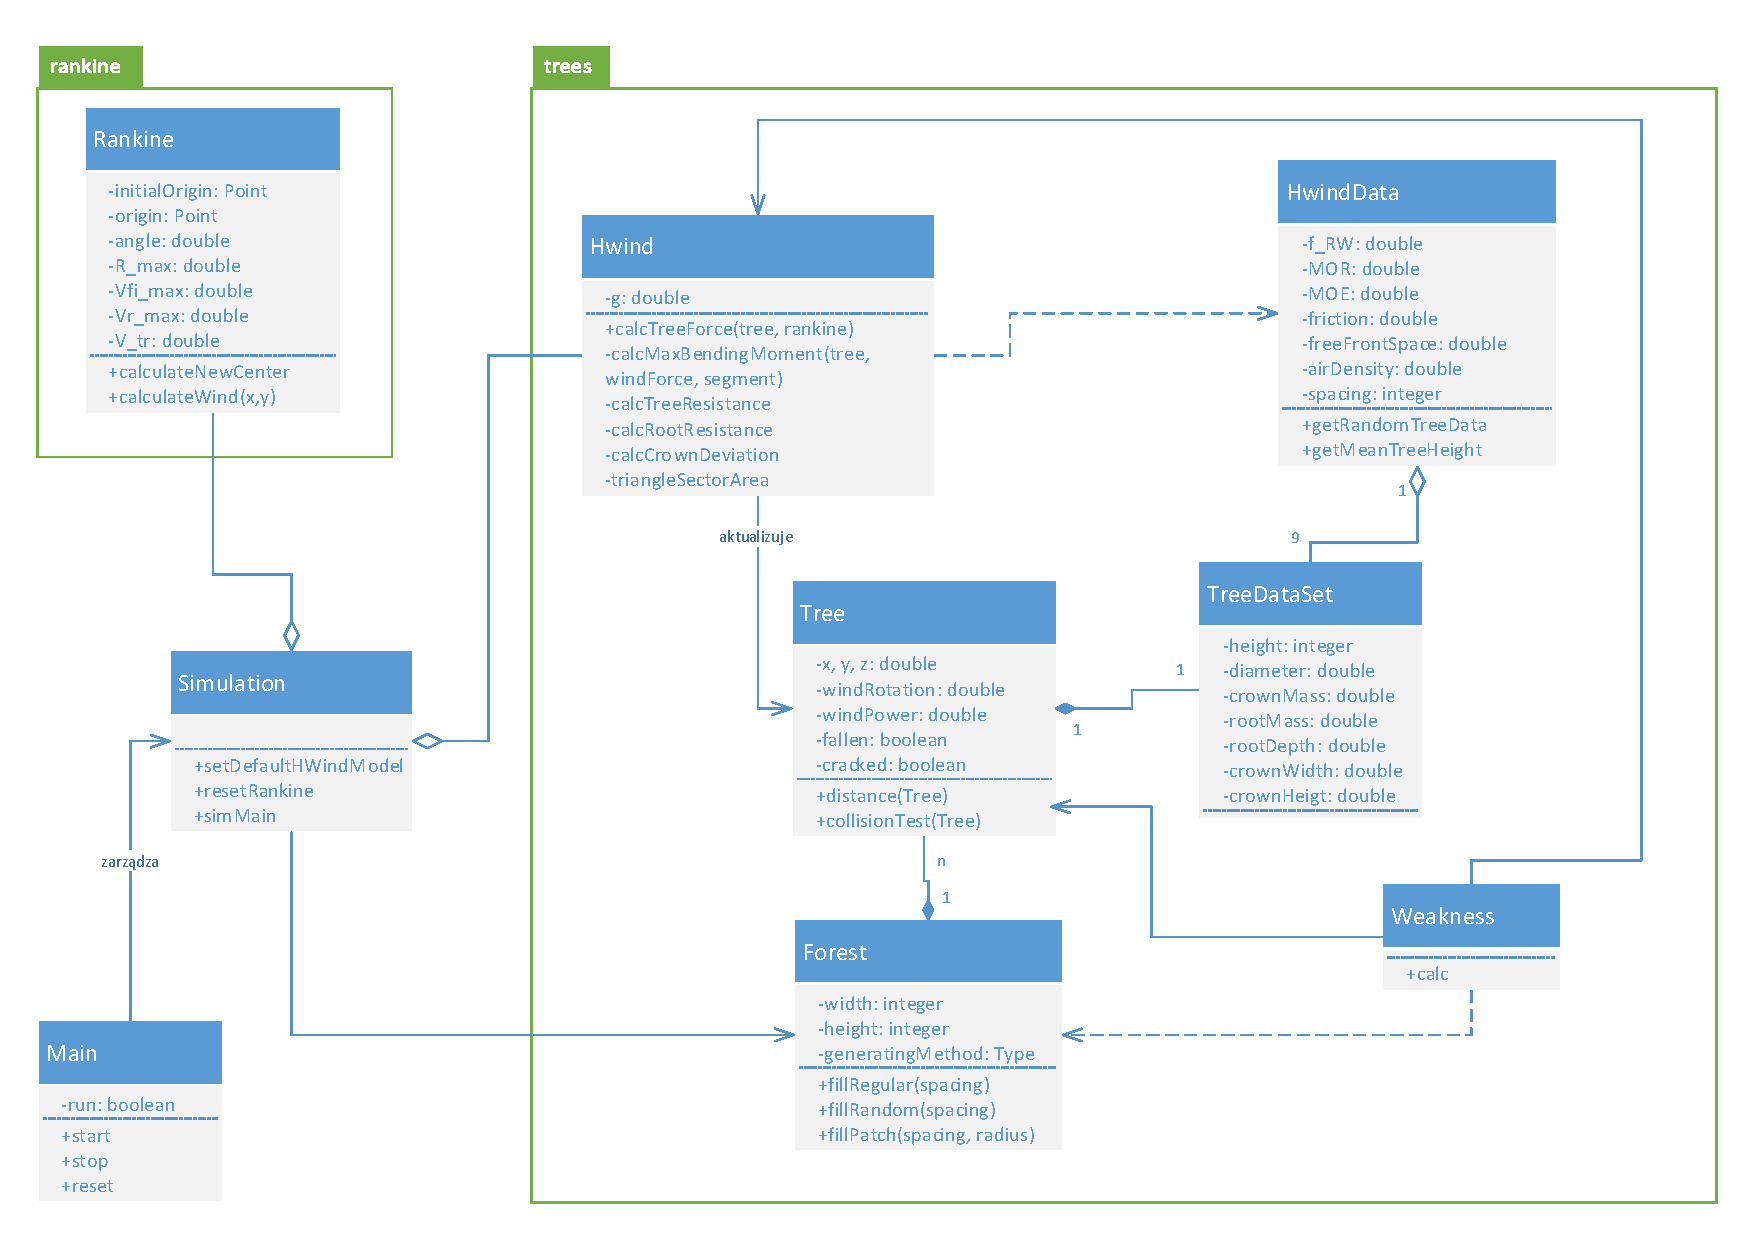
\includegraphics[scale=0.51]{uml}
	\caption{Diagram klas logiki aplikacji.}
	\label{fig:uml1}
\end{figure} 

Aplikacja została zaimplementowana w języku Java. 

Rysunek~\ref{fig:uml1} przedstawia zależności między klasami logiki aplikacji.

Głównymi klasami wpływającymi na przebieg symulacji są 
\begin{itemize}
\item Rankine (model wiru)
\item Hwind (model zniszczeń drzew)
\end{itemize}
Klasa Forest przechowuje informacje na temat parametrów lasu, takich jak jego wymiary, czy położenia drzew (przechowuje obiekty klasy Tree). Klasa Simulation stanowi element sterujący symulacji.
Klasy HwindData oraz TreeDataSet przechowują większość parametrów modelu zniszczeń drzew. Pierwsza posiada informacje średniej wysokości drzew w lesie, wartościach współczynnika tarcia oraz innych opisanych w charakterystyce modelu HWIND.
Druga z nich przechowuje informacje na temat konkretnego drzewa.

Klasa Weakness służy do wyznaczania wytrzymałości konkretnego drzewa w lesie na działanie siły wiatru (poprzez uwzględnienie jego sąsiedztwa).

Głównymi klasami które nas interesują z punktu widzenia użytkowników symulacji są klasy Tree i Forest. To one przechowują wynik symulacji.

 Rysunek~\ref{fig:uml2} przedstawia możliwe przypadki użycia. Aplikacja pozwala na przeprowadzenie symulacji zniszczeń, wraz z możliwością zmiany wartości jej parametrów. Działanie programu wizualizowane jest na bieżąco.

\begin{figure}[!h]
	\center
	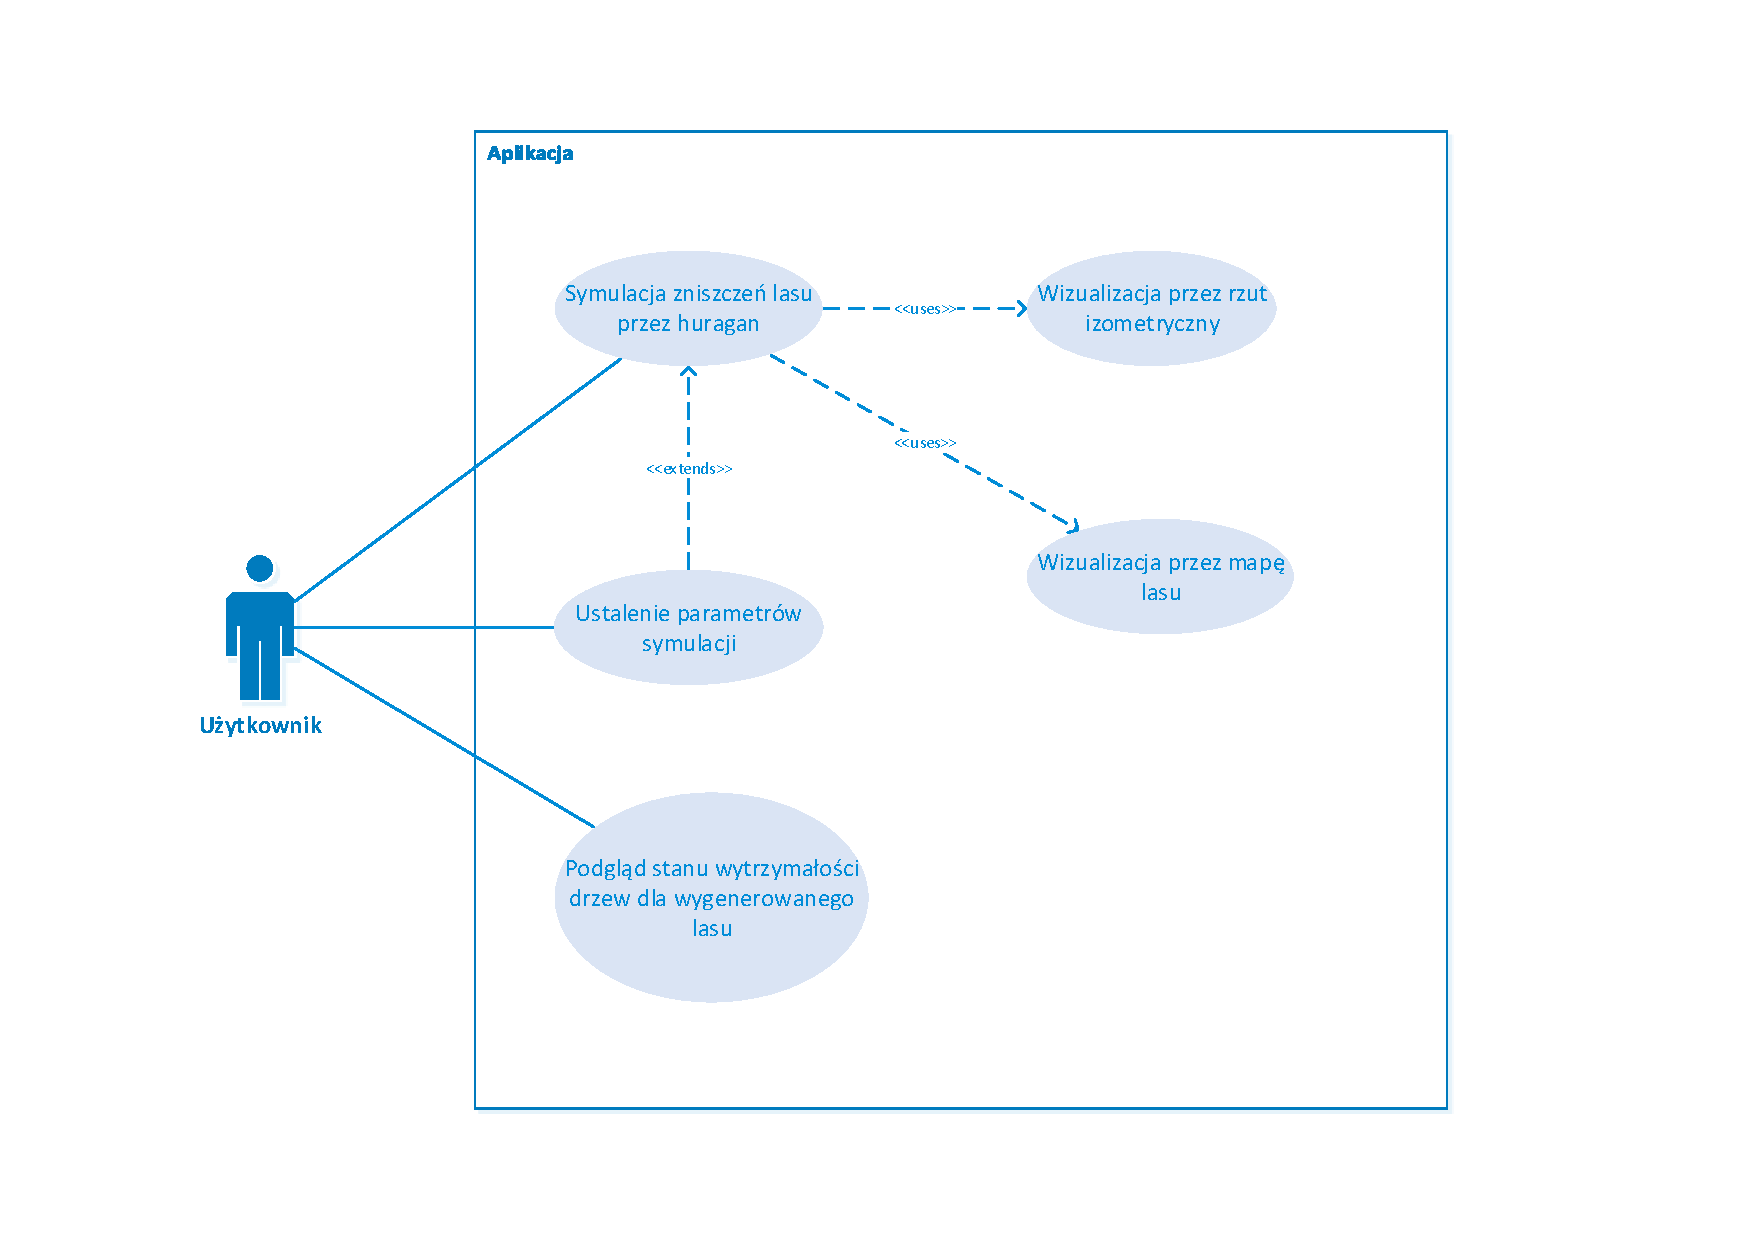
\includegraphics[scale=0.5]{uml_use_case}
	\caption{Diagram przypadków użycia.}
	\label{fig:uml2}
\end{figure} 

Zachowanie każdego drzewa zostało odzwierciedlone przez oddzielny wątek. Wykorzystując wzajemnie informacje o swym stanie, oraz obiekty klas modelu drzewa określają swój stan w danym momencie. Wykorzystanie koncepcji programowania agentowego pozwala na lepsze odzwierciedlenie rzeczywistej sytuacji, a co za tym idzie - uzyskania bardziej wiarygodnych wyników.





